\chapter{METODOLOGIA}

\section{Matlab}

MATLAB é um software interativo para computação numérica que possui uma série
de ferramentas, funções, visualisadores, ferramentas para debugging, estrutura de dados, 
entre outros auxilios que facilitam o desenvolvimento e o estudo de atividades
que utilizam a computação numérica. Por conta desses facilitadores, o MATLAB é
amplamente utilizado na indústria e no meio acadêmico.\cite{higham16}
Dada essa característica e a existência da função FMINCON a disposição
no ambiente MATBLAB, foi feita a escolha de se utiliza-lo para
a construção do código presente neste trabalho.

\subsection{fmincon}
Como o modelo matemático a ser otimizado é multivariável e 
possuindo restrições não-lineares, a função FMINCON do ambiente 
do MATLAB é utilizada para otimizar as variações de velocidade 
de forma a diminuir o erro de trajetória associado às 
flexibilidades do sistema que causam perturbações e vibrações 
indesejadas.
É uma função baseada em gradientes que busca por todos os 
mínimos locais de uma região que satisfaz outras restrições 
estipuladas \cite{albaghdadi21}.
Ela utiliza um conjunto de restrições superiores e inferiores 
para cada ponto e otimiza a função considerando as restrições 
estabelecidas pela função não linear, utilizando as equações de 
movimento para encontrar a solução da EDO de maneira a 
otimizar os parâmetros. Também permite uma série de configurações
incluindo a escolha de diferentes algorítimos de otimização entre
outros parâmetros sobre a função.

\section{Geração de Comando}

\subsection{Leitura Gcode}

Foi considerado no mapeamento do Gcode apenas comandos G1, extraindo
as informações dos eixos X, Y e do *feedrate* (F). Com base nesses valores
uma matriz 3 por n é criada, n sendo o número de comandos lidos do arquivo Gcode.

\section{lookahead}
Para a construção da curva de velocidade trapezoidal a partir da matriz de posições
e *feedrate* é necessário o cálculo das direções dos movimentos a serem realizados.
As direções são representadas por vetores unitários calculados a partir
do vetor deslocamento dividido pelo mesmo vetor normalizado (\ref{eq:dir_eq}). Sendo o vetor deslocamento
obtido pela diferença entre dois vetores de posição sequenciais.

\begin{equation}
    \label{eq:dir_eq}
    dir_{vector} = \frac{v}{norm(v)}
\end{equation}

Essas direções são utilizadas para o cálculo das velocidades pelo *look ahead*,
considerando os parâmetros de desvio máximo de junção ($\delta _{junc}$), que corresponde a distância máxima
entre o vertice da curva e a extremidade do raio e a aceleração maxima ($acc_{max}$) (figura \ref{fig:cornering}).
Importante ressaltar que se trata de um desvio virtual do caminho, utilizado para calcular a 
velocidade na curva ($v_{junc}$), que é calculada a partir da equação \ref{eq:v_jun}, enquanto o raio ($R$) é
calulado a partir da equação \ref{eq:R_jun}, considerando $\alpha$ como o ângulo entre os vetores
de velocidade, neste caso calculados a partir dos vetores de direção unitária ($dir_k$) (equação \ref{eq:alpha}) calculado na etapa anterior. 

\begin{equation}
    \label{eq:v_jun}
    v_{junc} = \sqrt{acc_{max}*R}
\end{equation}

\begin{equation}
    \label{eq:R_jun}
    R = \delta _{junc} \frac{sin\left(\frac{\alpha}{2}\right)}{1-sin\left(\frac{\alpha}{2}\right)}
\end{equation}

\begin{equation}
    \label{eq:alpha}
    sin\left(\frac{\alpha}{2}\right) = \left(\frac{norm(dir_1+dir_2)}{2}\right)
\end{equation}

Por fim, é necessário empregar uma lógica onde a velocidade de junta nunca seja maior
que a velocidade de entrada ou velocidade de saida. 

\subsection{Curva rapezoidal de velocidade}
A partir dessa matriz de posições e, agora também velocidades,
utilizamos a função responsável por gerar a curva trapezoidal de velocidades.

Essa função separa o deslocamento total do movimento em 3 fases de aceleração constante.
Na primeira fase a velocidade trazida da velocidade incial até a velocidade desejada
a aceleração constante, na segunda fase a velocidade é mantida constante na velocidade desejada
e por fim na terceira fase a velocidade é levada da velocidade desejada até a velocidade final.
Entretanto, em algumas situações pode não ser possível alcançar a velocidade desejada
e o perfil se limitar a duas fases, outras condições onde alguma das velocidades é igual a
velocidade desejada faz com que a quantidade de fases visiveis seja reduzida.

Para identificar se a velocidade desejada será alcançada é calculado a velocidade pico ($v_p$)
que é obtida extrapolando retas com as inclinações da aceleração na velocidade incial e final.
É possível obter a velocidade de pico através da equação \ref{eq:v_p}.

\begin{equation}
    \label{eq:v_p}
    v_p = \sqrt{\frac{(v_i^2+v_f^2)}{2}+acc*des_{tot}}
\end{equation}

A partir da comparação da velocidade pico com a velocidade desejada, indicada pelo *feedrate* disponibilizado no Gcode,
é possível determinar o padrão da curva de velocidade deste movimento.
Caso a velocidade de pico for maior do que a velocidade desejada, temos 3 fases de deslocamento
que podem ser calculadas pelas equações \ref{eq:des_seg_acc} e \ref{eq:des_seg_no_acc}.
Caso a velocidade de pico seja igual ou menor do que a velocidade desejada, teremos 2 fases de deslocamento
que são calculadas a partir da equação \ref{eq:des_seg_acc}.

\begin{equation}
    \label{eq:des_seg_acc}
    des_{segment} = \frac{(v_f^2-v_i^2)}{(2*acc_{segment})}
\end{equation}

\begin{equation}
    \label{eq:des_seg_no_acc}
    des_{middle} = des_{total}-(des_{up}+des_{down})
\end{equation}

É possível calcular também os intervalos de tempo dessas fases, através das 
equações \ref{eq:dt_seg_acc} e \ref{eq:dt_seg_no_acc}.

\begin{equation}
    \label{eq:dt_seg_acc}
    dt_{segment} = \frac{(v_f-v_i)}{acc_{segment}}
\end{equation}

\begin{equation}
    \label{eq:dt_seg_no_acc}
    dt_d = \frac{des_d}{v_d}
\end{equation}

Além disso é calculado a variação de velocidade nos intervalos pela equação \ref{eq:delta_vel}.

\begin{equation}
    \label{eq:delta_vel}
    \Delta vel = v_f-v_i
\end{equation}

Esses passos resultam em uma nova matriz contendo informações
sobre o a variação da posição, do tempo, da velocidade e sobre a aceleração e 
direção de deslocamento nos pontos iniciais e finais do Gcode e também nos pontos
onde existe uma alteração na aceleração.

\subsection{Interpolação}

A partir dessa matriz, é utilizada uma função de interpolação para dividir cada intervalo dessa matriz em intervalos menores
baseados em um passo de tempo definido para esta interpolação.
Assim criando-se uma nova matriz dos dados interpolados.
Para se dividir esses intervalos é possível utilizar a equação \ref{eq:N_steps}
calculando o número de passos neste intervalo, anexando à matriz os passos de tempo e por fim
o restante do intervalo, calculado pela equação \ref{eq:dt_interpol_last_step}.
Com base nestes passos de tempo, é possível calcular o deslocamento para cada um destes passos
através da equação \ref{eq:delta_des_interpol}.

\begin{equation}
    \label{eq:N_steps}
    N_{steps} = \lceil\frac{\Delta t_i}{\Delta t_{step_{size}}}-1\rceil
\end{equation}

\begin{equation}
    \label{eq:dt_interpol_last_step}
    \Delta t_{last_{step}}= \Delta t_i - \Delta t_{step_{size}}*N_{steps} 
\end{equation}

\begin{equation}
    \label{eq:delta_des_interpol}
    \Delta des_i = \Delta v_i*\Delta t_i+ \frac{acc_{segment}*\Delta t_i^2}{2} 
\end{equation}

A partir dos vetores de direção e da função acumuladora que se consite em acumular os valores de um vetor.
Obtemos uma matriz de posições, velocidades e tempo.

\begin{equation}
    \label{eq:acumulator_function}
    \begin{split}
        v_{0} &= init_{value} + v_{0} \\
        v_k &= v_k+v_{k-1}
    \end{split}
\end{equation}

% \section{Runge Kutta}



% s(:,1) = s0;
    
%     A = A_model;
%     B = B_model;
%     N = length(t)-1;
%     for i=1:N
%         dt(i) = t(i+1)-t(i);
%         uhalf = u_t_interpolator(u(:,i),u(:,i+1),dt(i),dt(i)/2);

%         k1(:,i) = dynamic_model(s(:,i),u(:,i),A,B);
%         k2(:,i) = dynamic_model(s(:,i)+k1(i)*dt(i)/2,uhalf,A,B);
%         k3(:,i) = dynamic_model(s(:,i)+k2(i)*dt(i)/2,uhalf,A,B);
%         k4(:,i) = dynamic_model(s(:,i)+k3(i)*dt(i),u(:,i+1),A,B);

%         avg_dot = (k1(:,i) + 2*k2(:,i) + 2*k3(:,i) + k4(:,i))/6;
%         s(:,i+1) = s(:,i) + dt(i)*avg_dot;
%     end


% Para o calculo da estimativa da respota do sistema, utilizamos a função Runge Kutta
% Primeiramente calculamos os valores de k1,k2,k3 e k4, calculamos a média da derivada do vetor de variaveis
% e por fim o calculo do vetor x.



\section{Modelagem dinâmica de uma impressora 3D}
Para a modelagem do sistema mecânico são consideradas as seguintes simplificações:
\begin{itemize}
    \item Não existe escorregamento nem perda de potência na interação entre a polia e a correia
    \item A correia apresenta um comportamento equivalente à uma mola e um amortecedor em paralelo
    \item O bico injetor é um corpo rígido uniforme de geometria simples
    \item A correia está acoplada nos dois lados da peça que se movimenta nos trilhos, entretanto como a correia só permite o tensionamento ela será considerada como um conjunto mola amortecedor simples
\end{itemize}

Para a modelagem dinâmica dos eixos X e Y da impressora 3D, 
é considerado que os eixos são completamente independentes, 
a flexibilidade da correia é aproximada utilizando um conjunto 
mola amortecedor e a transmissão de movimento e torque dos 
motores é considerada como ideal e não será abordada.
Assim duas posições de estudo surgem para cada eixo, uma delas 
representa a posição ideal, caso o sistema não possuiesse nenhuma flexibilidade
ou perda, que também é a posição desejada pelo usuário ($px_b$). 
A segunda posição considera as forças inerciais e a 
flexibilidade introduzida pela correia, ou seja, a posição real simulada pelo modelo
e no caso empírico a posição real ($px$) como na figura \ref{fig:din_model}.


\begin{figure}[!htb]
    \centering
    \caption{Visualização das posições do sistema}
    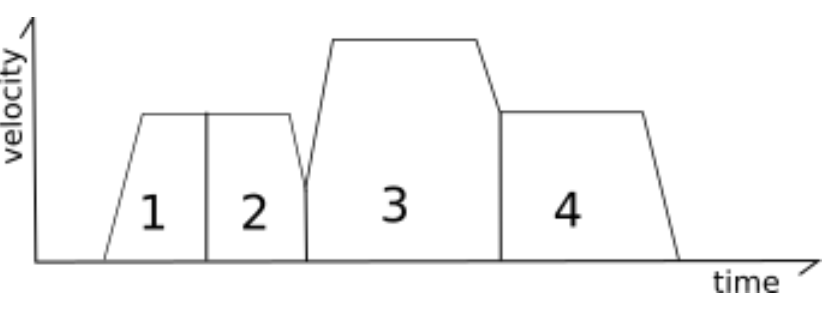
\includegraphics[scale=0.4]{trapezoidex}

    \label{fig:din_model}
\end{figure}

\begin{multline}
    \label{eq:mov_impressora}
    m \ddot{px} + c(\dot{px} - \dot{px_b}) + k(px-px_b) = 0 \\
    \ddot{px}  = - \frac{c}{m}(\dot{px} - \dot{px_b}) - \frac{k}{m}(px-px_b) \\
    \ddot{px}  = - \frac{c}{m} \dot{px} + \frac{c}{m} \dot
    {px_b} - \frac{k}{m} px + \frac{k}{m} px_b \\
    \ddot{px}  = - \frac{c}{m} \dot{px} - \frac{k}{m} px + \frac{c}{m} \dot{px_b} + \frac{k}{m} px_b
\end{multline}

\subsection{Espaço de estados}
A formulação de espaço de estados foi utilizada com intuito de facilitar as operações e
a a solução do sistema, dado sua característica de dividir uma equação diferencial
de ordem superior em um sistema de equações diferenciais de ordem 1.
O modelo dinâmico do sistema é apresentado na formulação de espaço de estados 
na equação \ref{eq:espaco_de_estados_din_model}, baseado na equação \ref{eq:mov_impressora},
utilizando a mesma equação para a base do eixo y.

\begin{equation}
    \label{eq:espaco_de_estados_din_model}
    \begin{bmatrix}
        \dot{px} \\
        \ddot{px} \\
        \dot{py} \\
        \ddot{py}
    \end{bmatrix}
    =
    \begin{bmatrix}
        0 & 1 & 0 & 0 \\
        -\frac{k_x}{m_x} & -\frac{c_x}{m_x} & 0 & 0 \\
        0 & 0 & 0 & 1 \\
        0 & 0 & -\frac{k_x}{m_x} & -\frac{c_x}{m_x}
    \end{bmatrix}
    \begin{bmatrix}
        px \\
        \dot{px} \\        
        py \\
        \dot{py} \\
    \end{bmatrix}
    +
    \begin{bmatrix}
        0 & 0 & 0 & 0 \\
        \frac{k_x}{m_x} & \frac{c_x}{m_x} & 0 & 0 \\
        0 & 0 & 0 & 0 \\
        0 & 0 & \frac{k_x}{m_x} & \frac{c_x}{m_x}
    \end{bmatrix}
    \begin{bmatrix}
        px_b \\
        \dot{px_b}  \\
        py_b \\
        \dot{py_b} 
    \end{bmatrix}
\end{equation}

Em uma notação simplificada temos a equação \ref{eq:simp_state_space_din_model}
\begin{equation}
    \label{eq:simp_state_space_din_model}
    \dot x = A*x+B*u
\end{equation}

\section{Otimização FMINCON}
\subsection{Restrições lineares e limites de borda}
Não foi utilizado nenhuma restrição linear nessa otimização.
Os limites superiores (upperbound) e inferiores (lowerbound) foram definidos
baseados nos limites físicos da impressora para as posições x, xb e y,yb, 
enquanto os limites para o vetor de variação de tempo foi estipulado uma margem
configuravel baseada no próprio vetor de variação do tempo.
Estas definições estão representadas pelo conjunto de equações \ref{eq:ublb_eqs}.

\begin{equation}
    \label{eq:ublb_eqs}
    \dot x = A*x+B*u
\end{equation}

% N = length(x(5,:));
% base = ones(1,N);

% lb(1,:) = base*min_x;
% lb(2,:) = base*min_y;
% lb(3,:) = base*min_x; % des_ux
% lb(4,:) = base*min_y; % vel_ux
% lb(5,:) = base*-0.0002;

% ub(1,:) = base*max_x;
% ub(2,:) = base*max_y;
% ub(3,:) = base*max_x; 
% ub(4,:) = base*max_y; 
% ub(5,:) = (x(5,:)+0.0002)*1.2;

\subsection{Restrições não lineares}

************************************
Blocked
************************************


% t = x(5,:);

% des_x = x(1,:);
% des_y = x(2,:);
% vel_x(1) = 0;
% vel_y(1) = 0;
% acc_x(1) = 0;
% acc_y(1) = 0;

% des_xb = x(3,:);
% des_yb = x(4,:);
% vel_xb(1) = 0;
% vel_yb(1) = 0;
% acc_xb(1) = 0;
% acc_yb(1) = 0;

% %dv = des/dt; da = dv/dt ; 
% %des = vi*t+at^2/2; a = 2*(des/t-vi)/t
% % Vf^2-Vi^2 = 2ades

% ceq=[des_x(1),des_y(1),t(1), des_xb(1), des_yb(1)];    
% c=[];

% for i = 1 : (length(t)-1)
%     dt = t(i+1)-t(i);
    
%     delta_x = (des_x(i+1)-des_x(i));
%     delta_y = (des_y(i+1)-des_y(i));
    
%     acc_x(i+1) = 2*((delta_x/dt)-vel_x(i))/dt; 
%     acc_y(i+1) = 2*((delta_y/dt)-vel_y(i))/dt;
%     vel_x(i+1) = vel_x(i)+acc_x(i+1)*dt;
%     vel_y(i+1) = vel_y(i)+acc_y(i+1)*dt;

%     delta_xb = (des_xb(i+1)-des_xb(i));
%     delta_yb = (des_yb(i+1)-des_yb(i));
    
%     acc_xb(i+1) = 2*((delta_xb/dt)-vel_xb(i))/dt;
%     acc_yb(i+1) = 2*((delta_yb/dt)-vel_yb(i))/dt;
%     vel_xb(i+1) = vel_xb(i)+acc_xb(i+1)*dt;
%     vel_yb(i+1) = vel_yb(i)+acc_yb(i+1)*dt;

%     AccelXb = abs((vel_xb(i+1)-vel_xb(i))/dt);
%     AccelYb = abs((vel_yb(i+1)-vel_yb(i))/dt);
    
%     c = [c max_acc-AccelXb max_acc-AccelYb];
    
%     x_i = [des_x(i);vel_x(i);des_y(i);vel_y(i)];
%     u_i = [des_xb(i);vel_xb(i);des_yb(i);vel_yb(i)];
    
%     f_i = A_model*x_i+B_model*u_i;
    
%     x_n = [des_x(i+1);vel_x(i+1);des_y(i+1);vel_y(i+1)];
%     u_n = [des_xb(i+1);vel_xb(i+1);des_yb(i+1);vel_yb(i+1)];
    
%     f_n = A_model*x_n+B_model*u_n;
    
%     x_c =(x_i+x_n)/2+dt*(f_i-f_n)/8;
%     u_c = (u_i+u_n)/2;
    
%     x_ca=-3*(x_i-x_n)/(2*dt)-(f_i+f_n)/4;
    
%     f_c = A_model*x_c+B_model*u_c;
    
%     delta = f_c-x_ca;
%     ceq=[ceq delta'];
% end
\subsection{Função objetivo (Objective Function)}
A função objetivo (FO) foi escolhida visando minimizar a diferença entre
as posições reais simuladas e a posição desejada pelo usuário.
Para isso, foi utilizada a equação \ref{eq:fo_eq}, onde seu resultado é
um escalar que quantifica o resultado do vetor a ser otimizado, permitindo
que o algoritimo procure alterar os valores do vetor, sem quebrar suas restrições e limites,
de maneira a minizar o resultado da FO.

\begin{equation}
    \label{eq:fo_eq}
    Ob = (x - x_{desejado})*(x - x_{desejado})'+(y - y_{desejado})*(y - y_{desejado})'
\end{equation}

\subsection{Cofiguração da Fmincon}
Foi utilizado as seguintes configurações da função fmincon:

**configurações**

\begin{table}
    \begin{center}
    \caption{Tabela de parâmetros opcionais da FMINCON}
    \label{tab:fmincon_options}
    \begin{tabular}{c c}
        Opção & Valor \\ \hline
        TolFun & 0.000000001 \\
        MaxIter & 100000 \\
        Display & iter \\
        DiffMinChange & 0.0001 \\
        Algorithm & interior-point \\
        StepTolerance & 1e-12 \\
        MaxFunEvals & 700000  \\ \hline
    \end{tabular}
    \end{center}
\end{table}

\section{Dados base e cofigurações}

aceleração máxima
desvio de junção
delta tempo
kx
ky
bx
by
mx
my

Levando em conta que modelo teste possui um comprimento de 20 cm e que os valores de rigidez e de amortecimento podem variar com a tensão aplicada, marca e tempo de uso, serão utilizados os valores aproximados para duas configurações (Tabela 2). A massa é estimada como sendo de 250 g que é uma estimativa com base nos conjuntos extrusora e hot end mais comuns.

\begin{table}
    \begin{center}
    \caption{Resultados experimentais dos coeficientes de rigidez e armortecimento de correias dentadas utilizadas em impressoras 3D}
    \label{tab:parametros_expe_belt}
    \begin{tabular}{c c c}
        teste & teste2 & teste3 \\ \hline
        1 & 2 & 3 \\
        4 & 5 & x+1 \\ \hline
    \end{tabular}
    \end{center}
\end{table}